\section{Model}

Consider a sequence of events $\mathcal{A} = (0,t_1, \ldots, t_M)$ arising from a nonhomogeneous Poisson process with  intensity $\lambda(t)$.
If the intensity is left continuous and piecewise constant with respect to a set of knots $\tau$ then the likelihood can be written
\begin{align}
\mathcal{L}(\mathcal{A}|\theta) &= \prod_{m=1}^M \lambda(t_m) \exp\left\{ - \int_{0}^{t_M} \lambda(s)ds \right\} \notag  \\
&= \prod_{m=1}^M \lambda(t_m) \prod_{k=1}^{|\tau|} \exp\left\{ - (\tau_{k} - \tau_{k-1}) \lambda(\tau_k) \right\}%  \exp\left\{ - (t - \tau_{M}) \lambda(t) \right\}
\end{align}
%{\color{red} (You've left out the right-censoring factor here (and also below).)}

One can extend the above to marked point processes where each event contains additional information.
In the context of relational events occurring among $N$ nodes, each event in the process contains both a sender $i$ and a recipient $j$ such that  $(i,j) \in \mathcal{R}$, where $\mathcal{R}$ is the \emph{risk set} comprised of all allowed dyads.
We assume each event involving dyad $(i,j) \in \mathcal{R}$ occurs as a Poisson process with intensity $\lambda_{ij}(t|\cdot)$ that is piecewise constant and depends on the previous history of events  $\mathcal{A}_t = \{(t_m,i_m,j_m): t_m \in [0,t) \}$.  
%The likelihood of an observed event history $\mathcal{A}$ extending from time 0 to the time of the final event, $t_M$, is 
The likelihood of an observed event history $\mathcal{A}_{t_M}$ (extending from time 0 to the time of the final event and denoted $\mathcal{A}$ for convenience) is
%The likelihood of an observed event history $\mathcal{A}_{t_M}$ (also denoted $\mathcal{A}$ for convenience) is
\begin{align}
\mathcal{L}(\mathcal{A}|\theta) &= \prod_{m=1}^M \lambda_{i_m,j_m}(t_m|\cdot) \prod_{(i,j) \in \mathcal{R}}\exp\{ - (t_m - t_{m-1}) \lambda_{ij}(t_m | \cdot) \}
\label{eqn:llk}
\end{align}

\begin{figure}
\centering
\begin{subfigure}[b]{0.45\linewidth}
  \begin{tikzpicture}[scale=.8,transform shape,thick]
    \node[vertex] (n1) at (0,0)  {1};
    \node[vertex] (n2) at (2,2)  {2};
    \node[vertex] (n3) at (4,0) {3};
    \node[vertex] (n4) at (2,-2) {4};
    \draw[-stealth] (.4,.4) -- (1.6,1.6);
    \draw[-stealth] (2.4,1.6) -- (3.6,.4);
    \node at (.7,1.1) {$t_1$};
    \node at (3.3,1.1) {$t_2$};
  \end{tikzpicture}
  \caption{Dynamic network data}
\end{subfigure}
\begin{subfigure}[b]{0.45\linewidth}
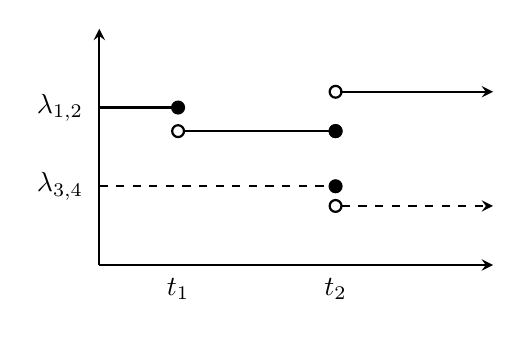
\begin{tikzpicture}[scale=1,transform shape,thick]
\draw[-stealth] (0,0) -- (0,3);
\draw[-stealth] (0,0) -- (5,0);

% First timeline
\draw (0,2) -- (1,2);
\draw[fill=black] (1,2) circle (0.75mm);
\draw (1,1.7) circle (0.75mm);
\draw (1.08,1.7) -- (3,1.7);
\draw[fill=black] (3,1.7) circle (0.75mm);
\draw (3,1.7) circle (0.75mm);
\draw (3,2.2) circle (0.75mm);
\draw[-stealth] (3.05,2.2) -- (5,2.2);

% second timeline
\draw[dashed] (0,1) -- (3,1);
\draw[fill=black] (3,1) circle (0.75mm);
\draw (3,.75) circle (0.75mm);
\draw[dashed, -stealth] (3.08,.75) -- (5,.75);

% labels
\node at (-.5,2) {$\lambda_{1,2}$};
\node at (-.5,1) {$\lambda_{3,4}$};
\node at (1,-.3) {$t_1$};
\node at (3,-.3) {$t_2$};
\end{tikzpicture}
\caption{Intensities for two dyads}
\end{subfigure}
\caption[]{Illustration of relational event data and the assumptions of the model.  (a) A sequence of two events among four nodes: (1,2) occurs at time $t_1$ and (2,3) occurs at time $t_2$. (b) The intensity functions $\lambda_{1,2}(t)$ (solid) and $\lambda_{3,4}(t)$ (dotted).  We assume $\lambda_{3,4}(t)$ can only change after events sent or received by node 3. }
\label{fig:example}
\end{figure}

{\color{red} (Need a better transition here.)}  We aim to learn about the dynamics between subsets of nodes.   To facilitate this, we assume each node $i$ belongs to latent cluster $z_i$ and use a log linear model for the intensity functions
\begin{align*}
\log \lambda_{ij}(t | \mathcal{A}_t,\mathbf{\beta},\mathbf{z}) &= \boldsymbol{\beta}'_{z_i,z_j} \mathbf{s}(t,i,j,\mathcal{A}_t)
%z_i &\sim \mbox{CRP}(\alpha) &
%\boldsymbol{\beta}_{k,l} &\sim %\mbox{N}_p(\boldsymbol{\mu},\boldsymbol{\sigma}^2I)
\end{align*}
where for each pair of clusters $(k,l)$ we have a parameter vector $\boldsymbol{\beta}_{k,l} \sim \mbox{N}_P(\boldsymbol{\mu},\boldsymbol{\sigma}^2I)$ that corresponds to the $P$-dimensional vector of statistics $\mathbf{s}(t,i,j,\mathcal{A}_t)$ computed from the previous history $\mathcal{A}_t$.
Thus, the rate of $(i,j)$ events has the same parameters as other events occurring between group $z_i$ and $z_j$.

% In practice we may believe an interaction between one dyad should not affect the rate of an entirely separate dyad.
As shown in Figure \ref{fig:example}, we only allow each intensity function $\lambda_{ij}(t)$ to change following an event where $i$ was the sender or the recipient.
This is sensible in distributed settings where $i$ has limited knowledge about interactions among other actors.
In the Supplementary Material we show how this assumption also reduces the computational complexity of computing the above likelihood.

We allow the blocks to share information by placing a hierarchical prior on the collection of $\boldsymbol{\beta}_{k.l}$ where $\mu_p \propto 1$ and $\sigma_p^2 \sim \mbox{Inv-Gamma}(\alpha_{\sigma},\beta_{\sigma})$.
The cluster assignments are given a non-parameteric prior $z_i \sim \mbox{CRP}(\alpha)$.
{\color{red} TODO: Expand on this?}

\subsection{Model specification}
\label{sec:specification}


Table \ref{tab:stats}  lists the statistics  $\mathbf{s}(t,i,j,\mathcal{A}_t)$ used in Section \ref{sec:experiments}.
For example, a particular node sending often may indicate they will continue to be a sender in the future.
We normalize these counts by the number of events up until a dyad's prior changepoint by using $f(x) = \log \frac{x+1}{m + N(N-1)}$. %\footnote{This seems to avoid ``explosion'' when simulating from the model.  TODO: Explore the theory about these sorts of statistics.  Aalen has a few suggestions.}
Other statistics could be of interest for particular substantive questions \cite{Butts2008,Vu2011}.  

% TODO: Awkward next sentence
The next set of statistics are \emph{participation shift} effects inspired by research in conversational norms \cite{Gibson2003}.
For example, an \texttt{ab-ba} effect indicates an increased propensity for reciprocity where the event $(a,b)$ is followed by $(b,a)$.
Though only the statistics in Table \ref{tab:stats} are used in our experiments, one may use any quantity that is computed using the previous history of events or known covariates about nodes or dyads.
The only restriction is that the statistic may not change in value between each observed event.\footnote{This prevents one from using the number of events occurring in some previous time window, as in \cite{Gunawardana2011}.}
% TODO: Also, need to be restricted to ego conditions if we want it fast

\subsection{Relation to other models}

Our formulation is reminiscent of the stochastic blockmodel \cite{Nowicki2001,Kemp2006} for static networks which models the probability of a dyad as $p(y_{ij}) =\mbox{logit}^{-1}( \eta_{z_i,z_j})$ where $\eta_{z_i,z_j}$ is interpreted as a mixing rate between group $z_i$ and group $z_j$.
In the proposed method, however, the blockmodel structure facilitates the study of intra-group and inter-group dynamics via a continuous-time network model.

The proposed family of models generalizes several important special cases.
For example,  using only the intercept statistic $s_0(t,i,j,\mathcal{A}_t) = 1$ is analogous to the stochastic block model for static networks.
Under this model each dyad is a homogeneous Poisson process and all dyad intensities $\lambda_{i,j}$ within block $(z_i,z_j)$ have the same intensity, $\exp\{\boldsymbol{\beta}_{z_i,z_j}\}$.
As these intensities do not change under this specification, the likelihood simplifies to
$$\mathcal{L}(\mathcal{A}|\beta) = \prod_{m=1}^M \lambda_{i_m,j_m} \prod_{(i,j) \in \mathcal{R}} \exp\{-t_M \lambda_{i,j}\}$$

Alternatively, if one models only the order of the events (ignoring the times at which they occur), the likelihood can be written as
\begin{align}
\mathcal{L}_{\mbox{mult}}(\mathcal{A}|\beta) = \prod_{m=1}^M \frac{\lambda_{i_m,j_m}(t_m | \cdot)}{\sum_{(i,j) \in \mathcal{R}} \lambda_{i,j}(t_m | \cdot)}.
\label{eqn:multllk}
\end{align}
The functional form is similar to conditional logit models used for discrete choice data \cite{McFadden1973}, though here the possible choices are all the dyads in $\mathcal{R}$.

\begin{table}[t]
\footnotesize
\center
\begin{tabular}{|l|l|}
\hline
Statistic & Formula\\
\hline
\hline
Intercept& $s_{0}(t,i,j,\mathcal{A}_t) = 1$\\
Reciprocity (AB-BA)& $s_{1}(t,i,j,\mathcal{A}_t) = I(i_m=i,j_m=j,i_{v_{mij}}=j,j_{v_{mij}}=i)$\\
Turn-continuing (AB-AY)& $s_{2}(t,i,j,\mathcal{A}_t) =  I(i_m=i,j_m=j,i_{v_{mij}}=i,j_{v_{mij}}\ne j)$\\
Turn-taking (AB-BY)&$s_{3}(t,i,j,\mathcal{A}_t) = I(i_m=i,j_m=j,i_{v_{mij}}=j,j_{v_{mij}}\ne i)$\\
%Turn-usurping (AB-XA)& $s_{7}(t,i,j) = I(i_m=i,j_m=j,i_{v_{mij}} \ne j,j_{v_{mij}}=i)$\\
%Turn-usurping (AB-XB)&$s_{8}(t,i,j) = I(i_m=i,j_m=j,i_{v_{mij}} \ne i,j_{v_{mij}}=j)$\\
Sender out-degree& $s_{4}(t,i,j,\mathcal{A}_t) = f(\sum_{m:t_m<t} I(i_m=i) )$\\
Sender in-degree& $s_{5}(t,i,j,\mathcal{A}_t) = f(\sum_{m:t_m<t} I(j_m=i) )$\\
Dyad count& $s_{6}(t,i,j,\mathcal{A}_t) = f(\sum_{m:t_m<t} I(i_m=i,j_m=j) )$\\
%Receiver out-degree& $s_{3}(t,i,j) = f(\sum_{m:t_m<t} I(i_m=j))$\\
%Receiver in-degree& $s_{4}(t,i,j) = f(\sum_{m:t_m<t} I(j_m=j))$\\
\hline
\end{tabular}
\caption{Statistics used to specify intensity functions using the previous history $\mathcal{A}_t$, where $v_{mij}$ is the index of the changepoint for $\lambda_{i,j}(t)$ previous to event $m$.}
\label{tab:stats}
\end{table}


\subsection{Related work}
Stochastic blockmodels have been extended to longitudinal network data
involving a sequence of networks occurring at discrete times
\cite{Ishiguro2010, Rodriguez2011}, while we focus on methods for
analyzing a stream of relational events. 
The proposed model is an extension of recent work on modeling event-based social network data using an event history approach \cite{Butts2008,Brandes2009,Perry2011,Stadtfeld2011,Opsahl2011,Vu2011,Vu2011a}. % \cite{AalenOddO.2008} 
Relational event models such as these require a knot at each observed event, while other approaches such as \cite{Gunawardana2011} learn the regions where an intensity is constant.
By using decision trees,  \cite{Gunawardana2011} also allow for a nonlinear relationship between statistics and intensity functions.  
We instead use latent variables to allow for heterogeneity in intensities across the set of possible events.

